\chapter{Message Authentication}
Fino a ora abbiamo parlato di sicurezza in termini di privacy. Tuttavia, soprattutto negli ultimi anni, è parecchio importante garantire autenticità poiché spesso la privacy non è necessaria. 

Il nostro obiettivo è quello di far sì che il mittente S, che vuole inviare un messaggio M al destinatario R, possa rendersi conto di eventuali corruzioni da parte di esterni; In questo modo verrebbero garantite autenticità e integrità del messaggio. 
Partiremo dal presupposto che S e R hanno una chiave segreta k in comune. L'autentica di un messaggio M produce un messaggio $M'$ che fa' sì che se R vede qualcosa di diverso da $M'$ si renda conto che il messaggio non è autentico.

\section{Message Authentication Codes}
Spesso $M'$ è proprio il messaggio M concatenato ad una stringa di lunghezza fissa detta \textbf{tag} che permetterà l'autenticazione del messaggio. Se l'autenticazione non va' a buon fine, il comportamento di R potrebbe variare in base al contesto; si potrebbero inviare messaggi di errore, si potrebbe interrompere la comunicazione ecc.\\
L'avversario parteciperà alla comunicazione e supporremo che questo abbia il pieno controllo di essa. 

A questo punto è lecito chiedersi se possa essere utile utilizzare gli strumenti già visti nei capitoli precedenti per ottenere autenticità. Banalmente, se S vuole mandare M a R, S calcola l'encryption del messaggio e poi r, una volta ricevuto lo decifrerà e, se il risultato ha "senso", allora lo dichiarerà come autentico. Intuitivamente questa cosa ha senso, se A non conosce M, non può nemmeno modificarlo in modo corretto. Tuttavia potremmo essere in grado di modificare il messaggio senza conoscerlo parzialmente o interamente. Ad esempio, se noi riuscissimo a cambiare c per far sì che 100 diventi 900, avremmo modificato il messaggio ma questo rimarrebbe di senso compiuto. 

Qui il problema non è quindi il cifrario utilizzato, semplicemente questi meccanismi sono stati progettati per scopi diversi, e quindi, su misura per specifiche diverse a quelle che stiamo cercando di ottenere adesso. È più opportuno nel nostro caso, creare su misura gli strumenti che ci saranno di aiuto. 

\section{MAC}
Per definire il MAC necessitiamo di questa serie di algoritmi:
\begin{itemize}
    \item \textbf{KeyGen:} questo algoritmo si occupa di restituire una stringa casuale.
    \item \textbf{MAC:} Prendiamo in input una chiave k, un messaggio $M \in \{0,1\}*$ e restituiamo un $tag \in \{0,1\} \cup Err$
    \item \textbf{VF:} Questo algoritmo è quello di verifica e non fa' altro che prendere in input k, M e un tag e restituisce 1 se la verifica va' a buon fine e 0 altrimenti.
\end{itemize}
Imponiamo che i verificatori siano deterministici poiché gestire destinatari a stati potrebbe diventare problematico a causa di problemi di sincronizzazione o di sicurezza della variabile stati. Eppure, non c'è dubbio che questi siano utili poiché, in certe situazioni, potrebbero prevenire attacchi di replay.  Nonostante ciò questi non verranno trattati in questo corso.

Considereremo, invece, sistemi \textbf{deterministici} che, se nei cifrari sembrano creare problemi, vedremo come qui saranno utili. Se il MAC è deterministico, avremo che l'algoritmo di verifica sarà sempre lo stesso, cioè: 
\begin{figure}[H]
    \centering
    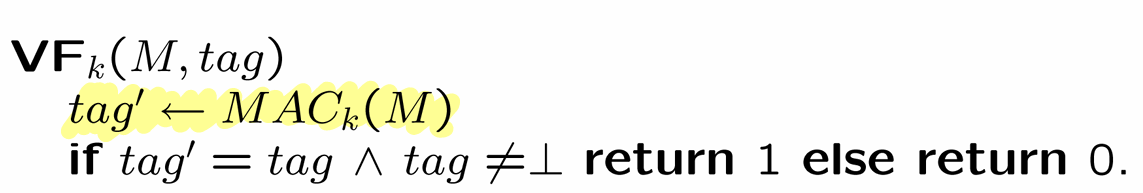
\includegraphics[width=0.7\linewidth]{Images/mac/verifica.png}
\end{figure}

\section{Modello di attaccante}
Dato che vogliamo dare una precisa definizione di sicurezza per quanto riguarda il MAC, possiamo lavorare come prima definendo innanzitutto un obiettivo e, successivamente, un attaccante adeguato.

Il nostro obiettivo sarà, quindi, quello di rilevare ogni tentativo di modifica da parte di A. E, per fare ciò, A cercherà di produrre dei \textbf{falsi} tali che $VF_k(M,tag)=1$. Per far sì che il nostro approccio sia il più generico possibile, non ci limiteremo a considerare solo messaggi che abbiano un senso, bensì qualunque tipo di messaggio poiché, se riusciamo a difenderci contro qualunque messaggio sia anche privo di senso, potremo farlo anche da messaggi con un senso. 

L'attaccante avrà in genere accesso a coppie $(M,tag)$ validi per cui lui potrà anche chiedere il tag di specifici messaggi m; chiameremo questo tipo di attacco $CMA$, cioè, chosen message attack. 
Possiamo anche definire il seguente esperimento a cui parteciperà l'attaccante:\footnote{UF sta per unforgiability}
\begin{figure}[H]
    \centering
    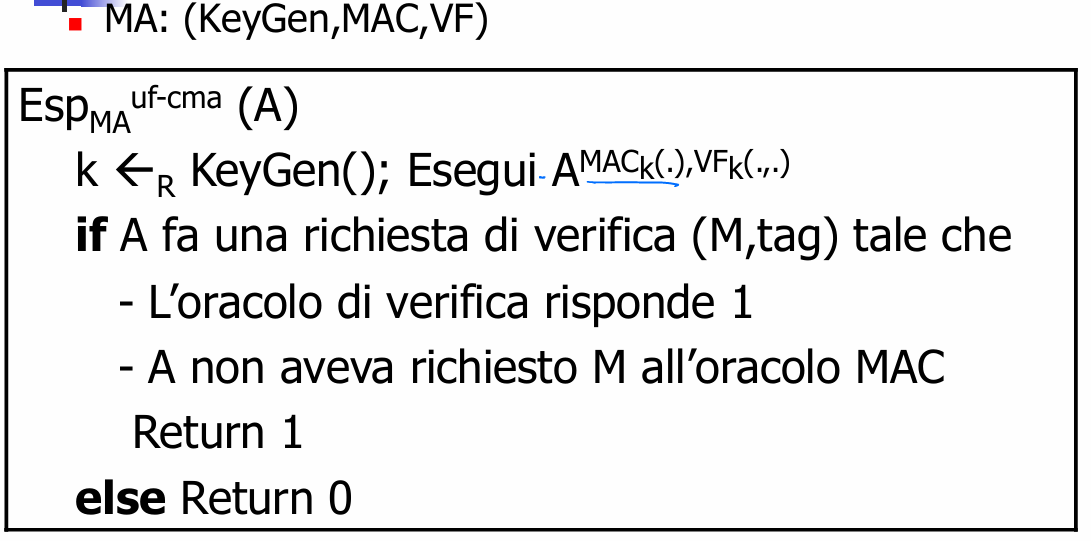
\includegraphics[width=0.7\linewidth]{Images/mac/esp_uf_cma.png}
\end{figure}

Qui faremo attenzione a due oracoli:
\begin{itemize}
    \item \textbf{MAC:} che prenderà un messaggio M e restituirà il tag associato.
    \item \textbf{VF:} che si occuperà di verificare se una coppia (messaggio, tag) sia corretta.
\end{itemize}

E diremo che un MA è sicuro se il vantaggio $Adv^{uf-cma}(A)$ è prossimo a 0:
\[Adv^{uf-cma}(A) = Pr[Esp_{MA}^{uf-cma}(A)=1]\]

È importante separare per i nostri scopi $q_s$ che rappresenta il numero di domande all'oracolo MAC e $q_v$ che rappresenta il numero di domande all'oracolo di verifica. Questo ci tornerà comodo per l'analisi che faremo successivamente.

Innanzitutto facciamo alcuni esempi di MAC non sicuri e vediamo quale è il problema. Ricordiamoci bene che il nostro obiettivo sarà quello di prevedere il MAC di un messaggio diverso da quelli che abbiamo già chiesto.
\begin{figure}[H]
    \centering
    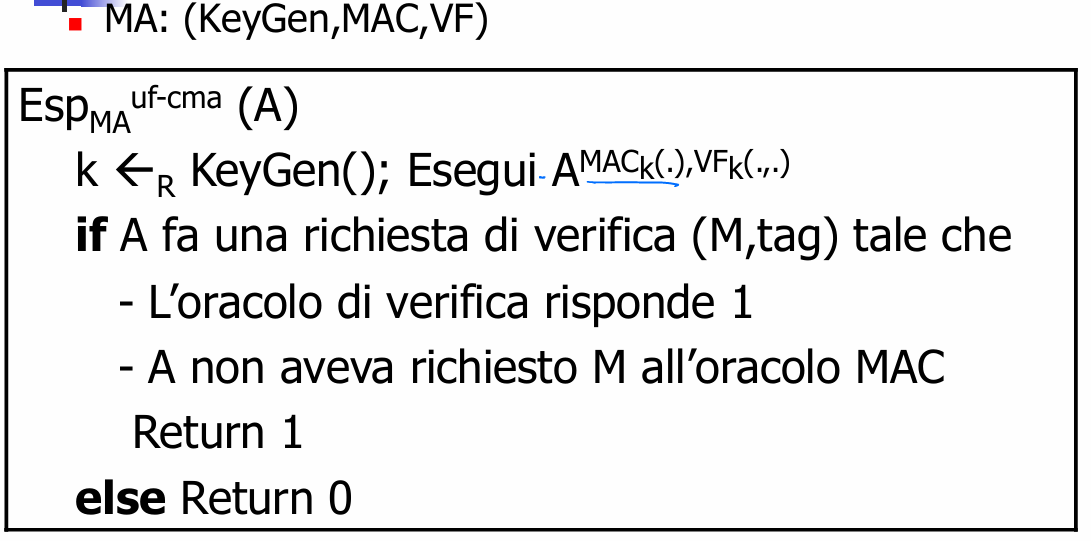
\includegraphics[width=0.7\linewidth]{Images/mac/esp_uf_cma.png}
\end{figure}

Per capire se è sicuro, possiamo ragionare allo stesso modo di come abbiamo fatto per le funzioni pseudo-random. Vediamo di costruire un attaccante che è in grado di prevedere il tag di un messaggio. 
\begin{figure}[H]
    \centering
    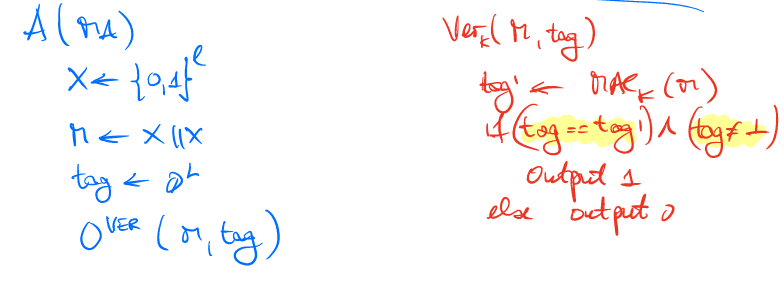
\includegraphics[width=0.7\linewidth]{Images/mac/esempio_unsec_attaccante.png}
\end{figure}
Oppure ancora:
\begin{figure}[H]
    \centering
    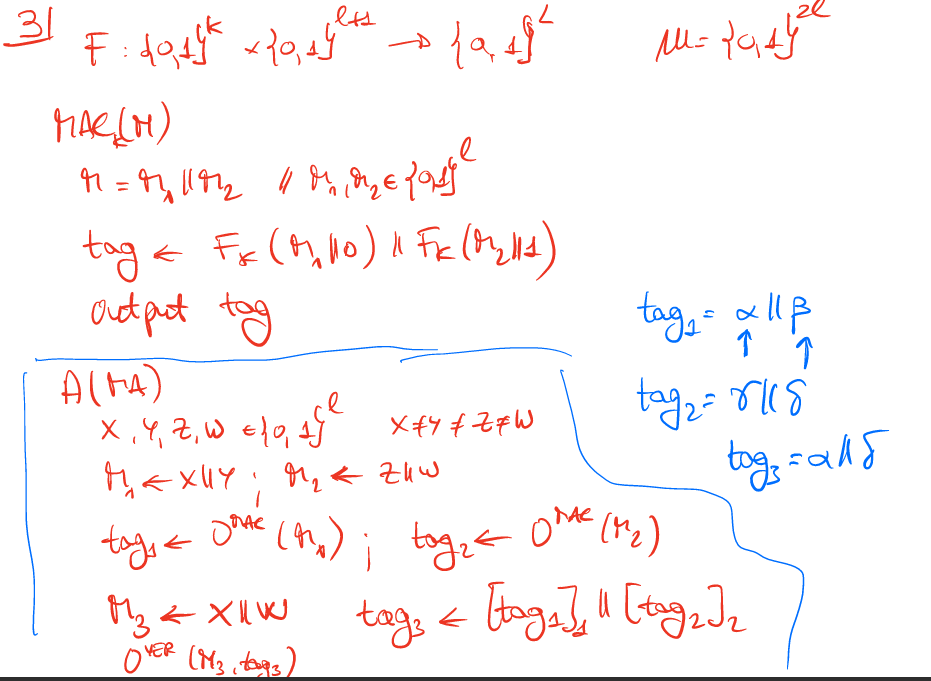
\includegraphics[width=0.7\linewidth]{Images/mac/esempio_2.png}
\end{figure}
Infine:
\begin{figure}[H]
    \centering
    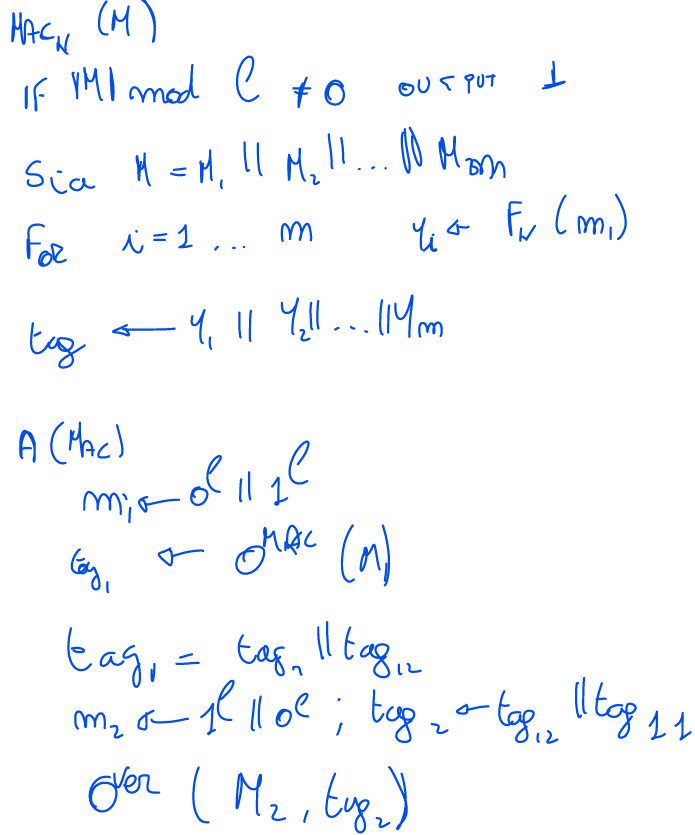
\includegraphics[width=0.5\linewidth]{Images/mac/esempio_3.png}
\end{figure}

\section{CBC-MAC}
Dagli esempi fatti, quello che sembra è che le prf non siano buone per costruire dei MAC sicuri, tuttavia, in realtà questo approccio è sicuro. Per fare ciò, banalmente si lavora a questo modo:
\begin{figure}[H]
    \centering
    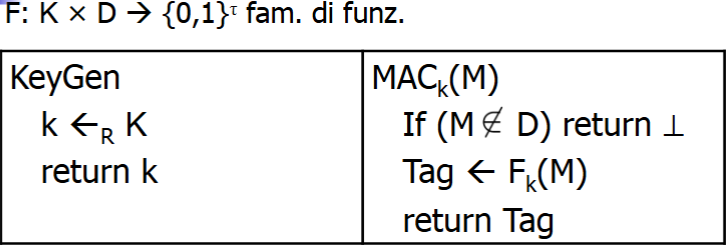
\includegraphics[width=0.7\linewidth]{Images/mac/mac_da_prf.png}
\end{figure}
Da qui abbiamo un teorema per cui:\\
Sia $F:K\times D \xrightarrow{} \{0,1\}^\tau$ una famiglia di funzioni, sia MA = (KeyGen, Mac) il metodo appena descritto. Preso A un avversario che attacca MA facendo $q_s + q_v$ domande, esiste un avversario B che attacca la prf che fa $q_s+q_v$ domande tale che:
\[Adv_{MA}^{uf-cma}(A)\leq Adv_{F}^{prf}(B)+\frac{q_v}{2^\tau}\]

Ciò vuole sostanzialmente dirci che possiamo rompere MA solo se rompiamo la prf sottostante. Costruiamoli:
\begin{figure}[H]
    \centering
    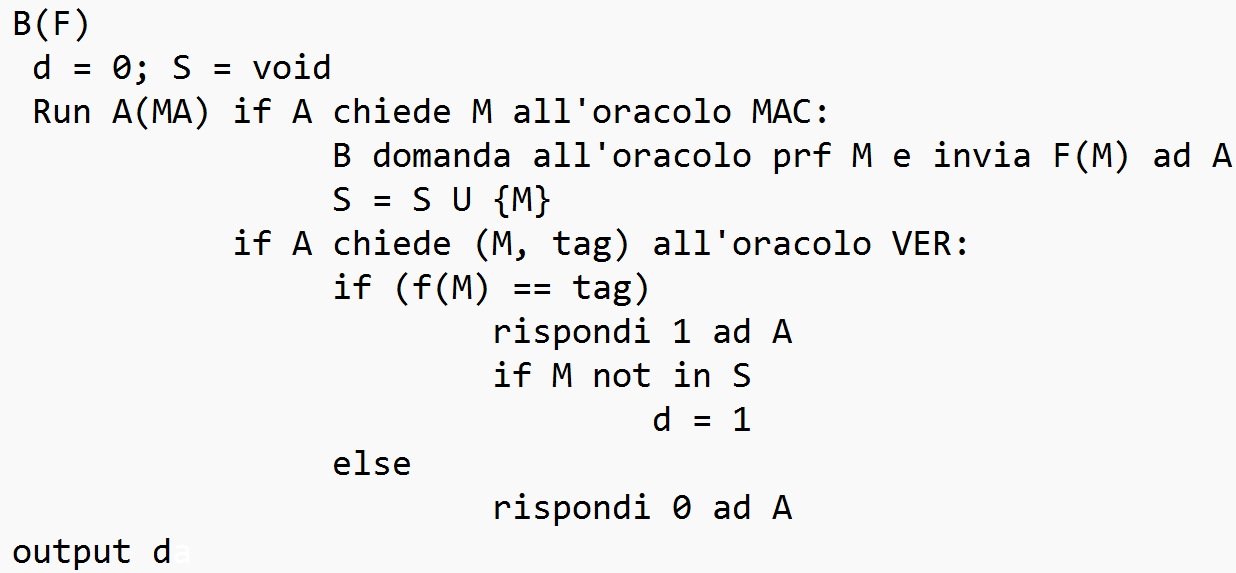
\includegraphics[width=0.7\linewidth]{Images/mac/dimostrazione_attaccante_B_A.png}
\end{figure}

Calcoliamo i vantaggi:
\begin{align*}
    &Adv(B)= Pr[Esp^{prf-1}(B)=1]-Pr[Esp^{prf-0}(B)=1]\\
    &Pr[Esp^{prf-1}(B)=1]= Adv(A)\\
    &Pr[Esp^{prf-0}(B)=1] = Pr[\tau_1 \lor \tau_2 \lor \dots \lor \tau_{qv}] \leq\\
    & \sum_{i}Pr[\tau_i]=\frac{q_v}{2^\tau}
\end{align*}
Il problema di questo tipo di utilizzi è il fatto che la cifratura di un messaggio genera un tag della stessa dimensione del messaggio per cui abbiamo un consumo di banda importante.

Un metodo più efficiente è quello chiamato \textbf{CBC-MAC} per cui a partire da un cifrario a blocchi $E:\{0,1\}^k \times \{0,1\}^n \xrightarrow{} \{0,1\}^n$ si costruisce il tag nel seguente modo:
\begin{figure}[H]
    \centering
    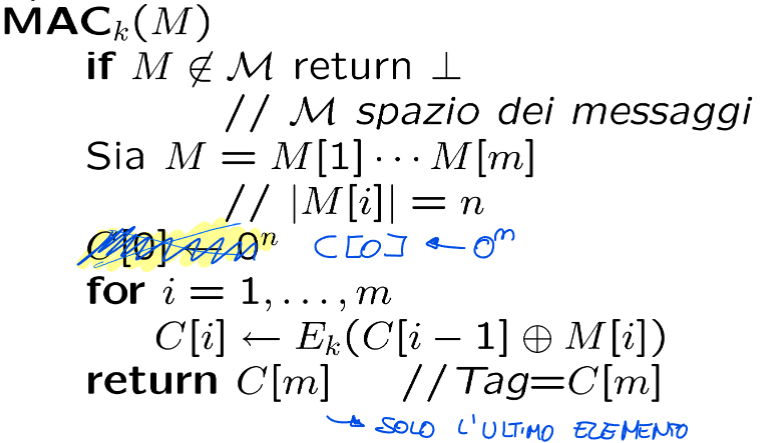
\includegraphics[width=0.5\linewidth]{Images/mac/mac_con_cbc.png}
\end{figure}

\textbf{Teorema}\\
Sia un cifrario a blocchi $E:\{0,1\}^k \times \{0,1\}^n \xrightarrow{} \{0,1\}^n$ e sia $\{0,1\}^{nm}$ lo spazio dei messaggi. Preso un avversario A contro CBC-MAC che fa q richieste di autentica e 1 richiesta di verifica, esisterà un avversario B che attacca E come PRP\footnote{Permutazione random dato che stiamo lavorando con un cifrario a blocchi} che fa q+1 domande tale che:
\[Adv_{MAC}^{uf-cma}(A)\leq Adv_E^{prp-cpa}(B)+\frac{m^2q^2}{2^{n-1}}\] 
In questo teorema, assumiamo che tutti i messaggi abbiano la stessa taglia e questo è necessario per la validità del teorema. Supponiamo che si possano prendere messaggi di lunghezza diversa:
\begin{figure}[H]
    \centering
    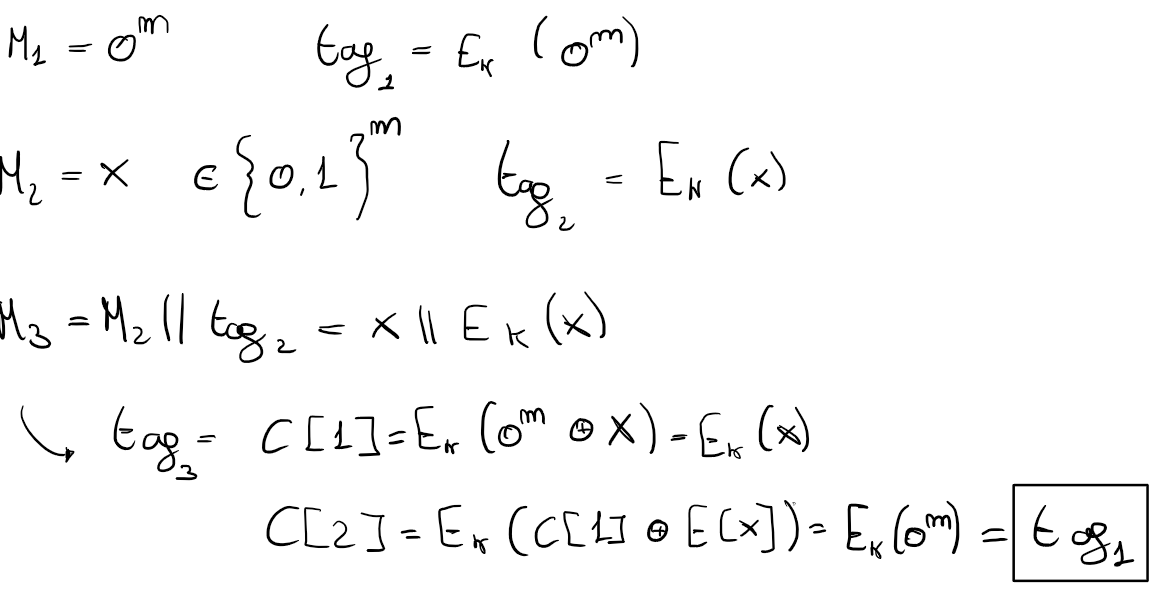
\includegraphics[width=0.7\linewidth]{Images/mac/dimostrazione_messaggi_l_diversa.png}
\end{figure}

Similmente, possiamo anche dimostrare che CBC-MAC randomizzato non è sicuro: 
\begin{figure}[H]
    \centering
    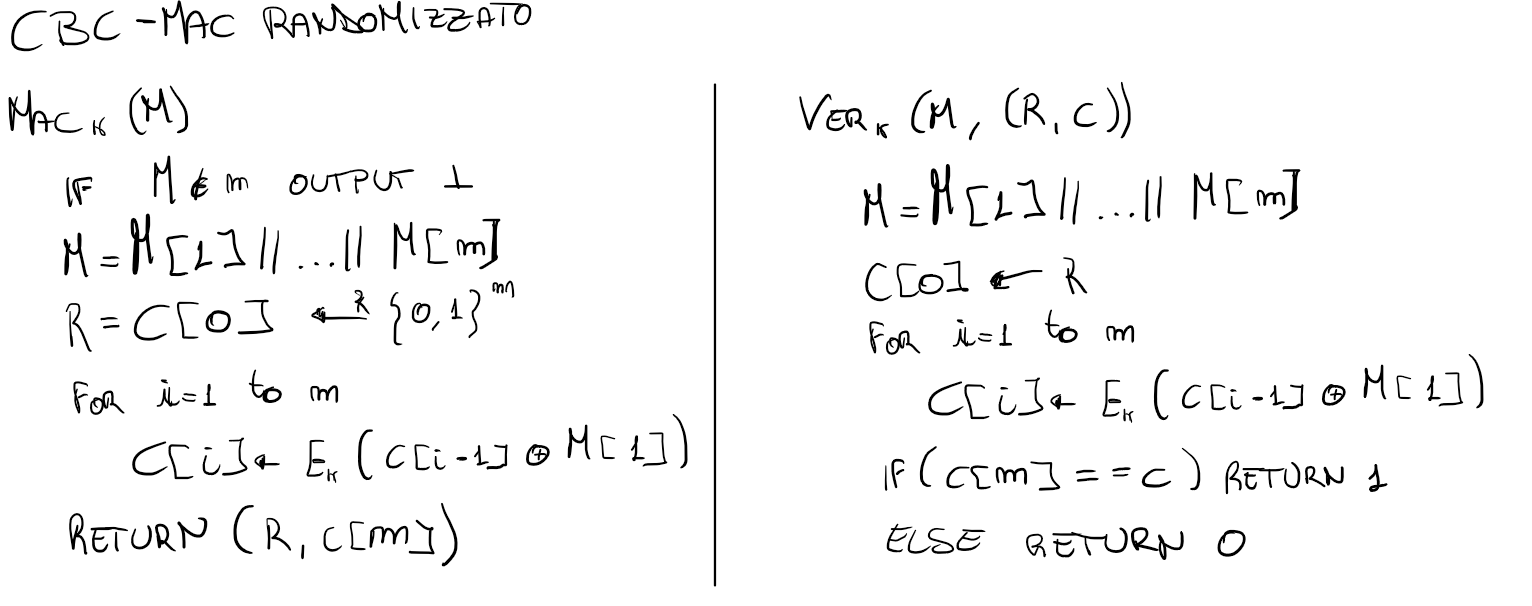
\includegraphics[width=0.7\linewidth]{Images/mac/cbc_mac_random.png}
\end{figure}
Il vero e proprio problema di questo metodo è che R, essendo randomizzato, deve essere obbligatoriamente rilasciato insieme al tag vero e proprio, dunque:
\begin{figure}[H]
    \centering
    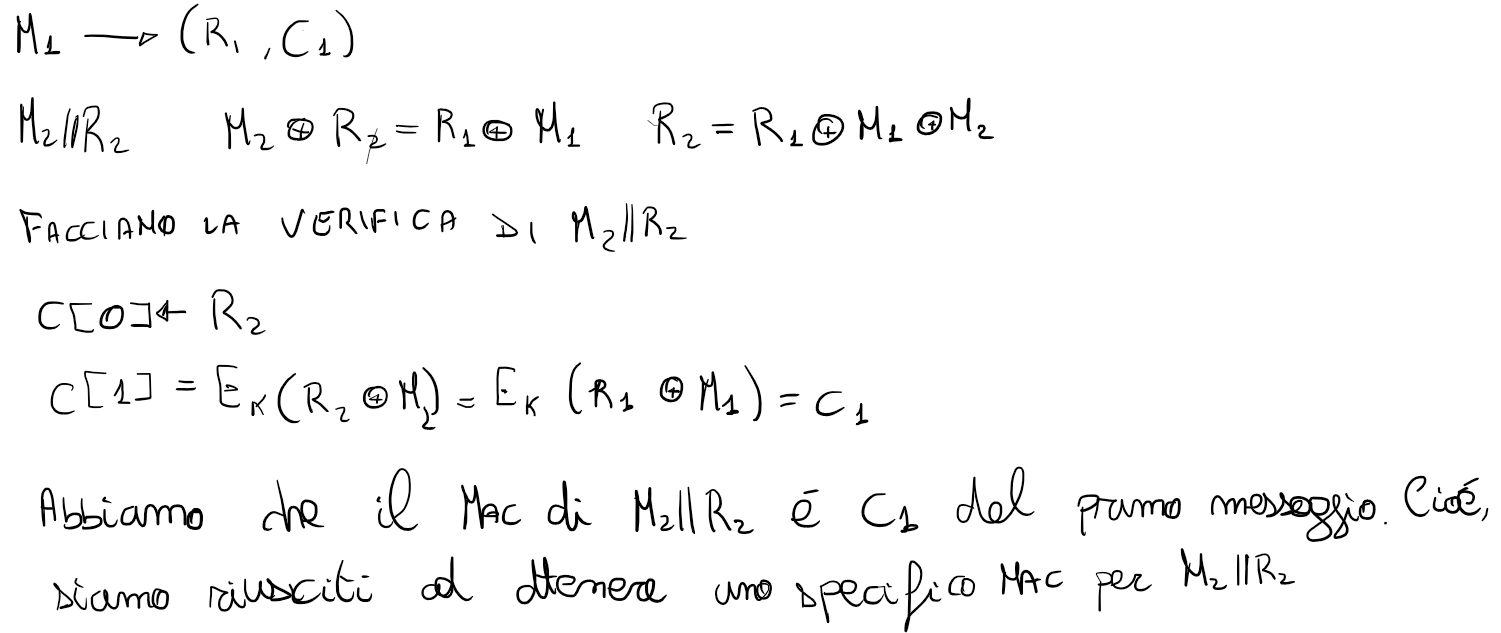
\includegraphics[width=0.7\linewidth]{Images/mac/attacco_cbc_mac_random.png}
\end{figure}
Il fatto che CBC-MAC sia deterministico è fondamentale per la sua sicurezza, poiché grazie a ciò, non è possibile replicare l'attacco precedente:
\begin{itemize}
    \item Quando l'attaccante riceve il tag per $M_1$, ottiene $tag_1 = E_k(0^n \oplus M_1)$.
    \item Se ora vuole falsificare un tag per $M_2$, dovrebbe calcolare $tag_2 = E_k(0^n \oplus M_2)$.
    \item Non può usare la tecnica di manipolazione dell'IV (perché l'IV è fisso e non può controllarlo) e, senza conoscere la chiave $k$, non può calcolare il risultato corretto.
\end{itemize}

Se volessimo ottenere CBC-MAC per messaggi a lunghezza variabile, avremo principalmente tre tipi di approcci:
\begin{enumerate}
    \item Utilizzare \textbf{chiavi indipendenti per messaggi di lunghezza diversa}. Questo approccio è banale, per ottenere chiavi diverse in base alla lunghezza potremmo fare a questo modo:
        \begin{align*}
            &k_l=F_k(l)\\
            &tag=CBC-MAC(k_l,m)
        \end{align*}
    \item Possiamo \textbf{prependere} a m la sua lunghezza così da non avere la necessità di fare un ulteriore calcolo dopo. Supponendo di voler effettuare l'attacco precedente, questo non sarebbe più fattibile poiché due messaggi di lunghezza diversa hanno due blocchi iniziali diversi e, quindi, nulla in comune.
    \item Possiamo utilizzare due \textbf{chiavi indipendenti} $k_1,k_2$ per poi fare:
        \begin{align*}
            &t=CBC-MAC(k_1, m)\\
            &tag=CBC-MAC(k_2, t)
        \end{align*}
    Anche in questo caso l'attacco non sarebbe replicabile perché le due iterazioni sono separate. Una cosa da segnalare è che la seconda iterazione di CBC è comunque fatta con un solo blocco e, quindi, molto più veloce della prima.
\end{enumerate}
\section{MAC da HASH (HMAC)}
Nonostante tutta la fatica fatta per ottenere CBC-MAC, questo è estremamente lento e, in pratica, quasi mai utilizzato. Al contrario, molto famosi sono i MAC ottenuti da funzioni hash costruite secondo la metodologia Markle-Damgard che hanno, come unico svantaggio, il dover assumere che la funzione di compressione abbia proprietà di pseudo casualità. 
Facciamo le seguenti ipotesi:
\begin{itemize}
    \item H, h restituiscono output di n bit.
    \item Se m è in $\{0,1\}^b$, $H(m)$ richiede una sola esecuzione di h.
    \item \textbf{IV, opad, ipad} sono costanti di lunghezza b. 
\end{itemize}

Vediamo quindi il funzionamento di \textbf{HMAC}:
\begin{figure}[H]
    \centering
    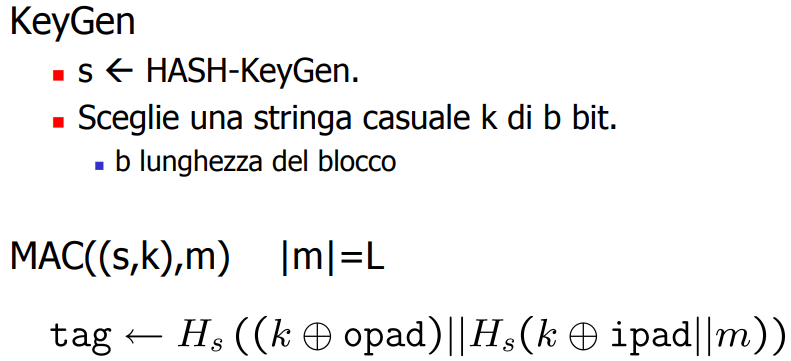
\includegraphics[width=0.7\linewidth]{Images/mac/hmac.png}
\end{figure}
Questa funzione è molto efficiente, facile da implementare e molto più sicura di tutte le altre funzioni non sicure adottate in commercio prima di questa standardizzazione.\\
Immaginiamo adesso di voler ottenere cifratura e autenticazione, le sole due cose possibili sono:
\begin{figure}[H]
    \centering
    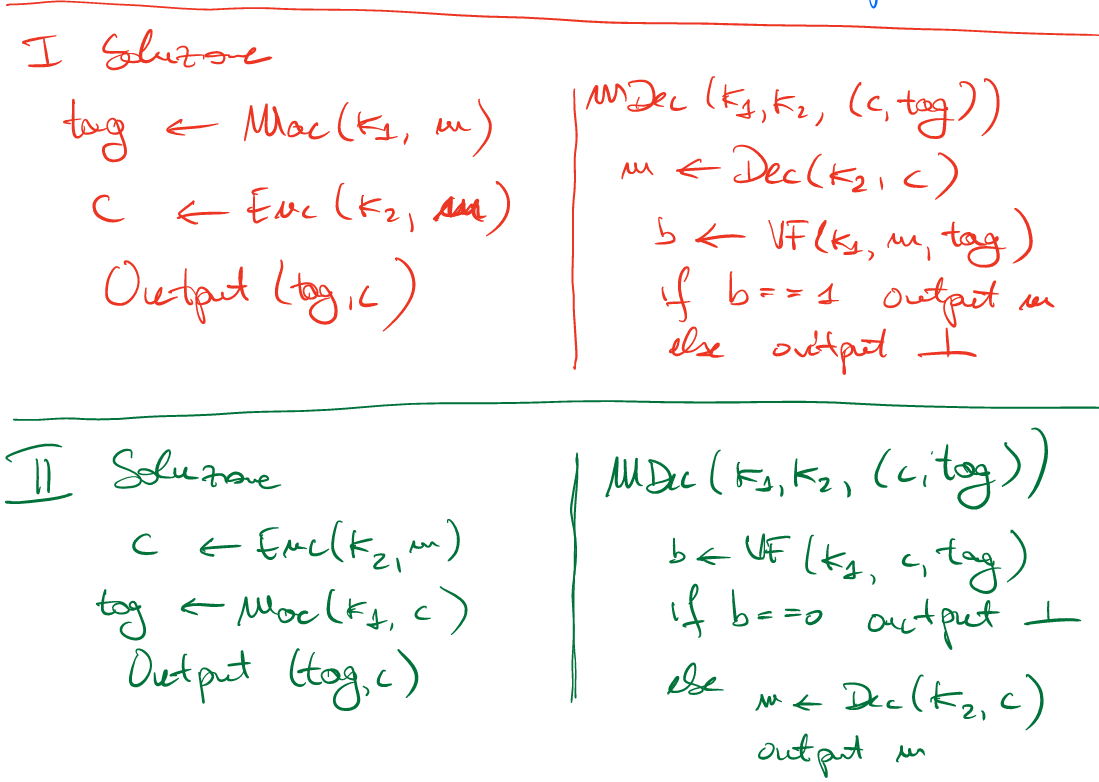
\includegraphics[width=0.7\linewidth]{Images/mac/cifratura_e_mac.png}
\end{figure}
Quindi, o facciamo prima la cifratura e poi calcoliamo il MAC oppure il contrario. Per quanto le cose sembrino apparentemente identiche, in realtà pensandoci bene non è sicuro effettuare prima il mac e poi la cifratura poiché inviando due volte lo stesso messaggio, il mac sarebbe lo stesso ma con la cifratura diversa. Facendo il contrario, essendo che la cifratura del messaggio cambia, cambia anche il suo mac, rendendo il secondo approccio sicuro rispetto all'altro.